\documentclass[12pt]{article}

\usepackage{tikz}
\usepackage{geometry}

\usetikzlibrary{mindmap}

\pagestyle{empty}

\geometry{landscape, margin=1cm}


\begin{document}
\begin{center}
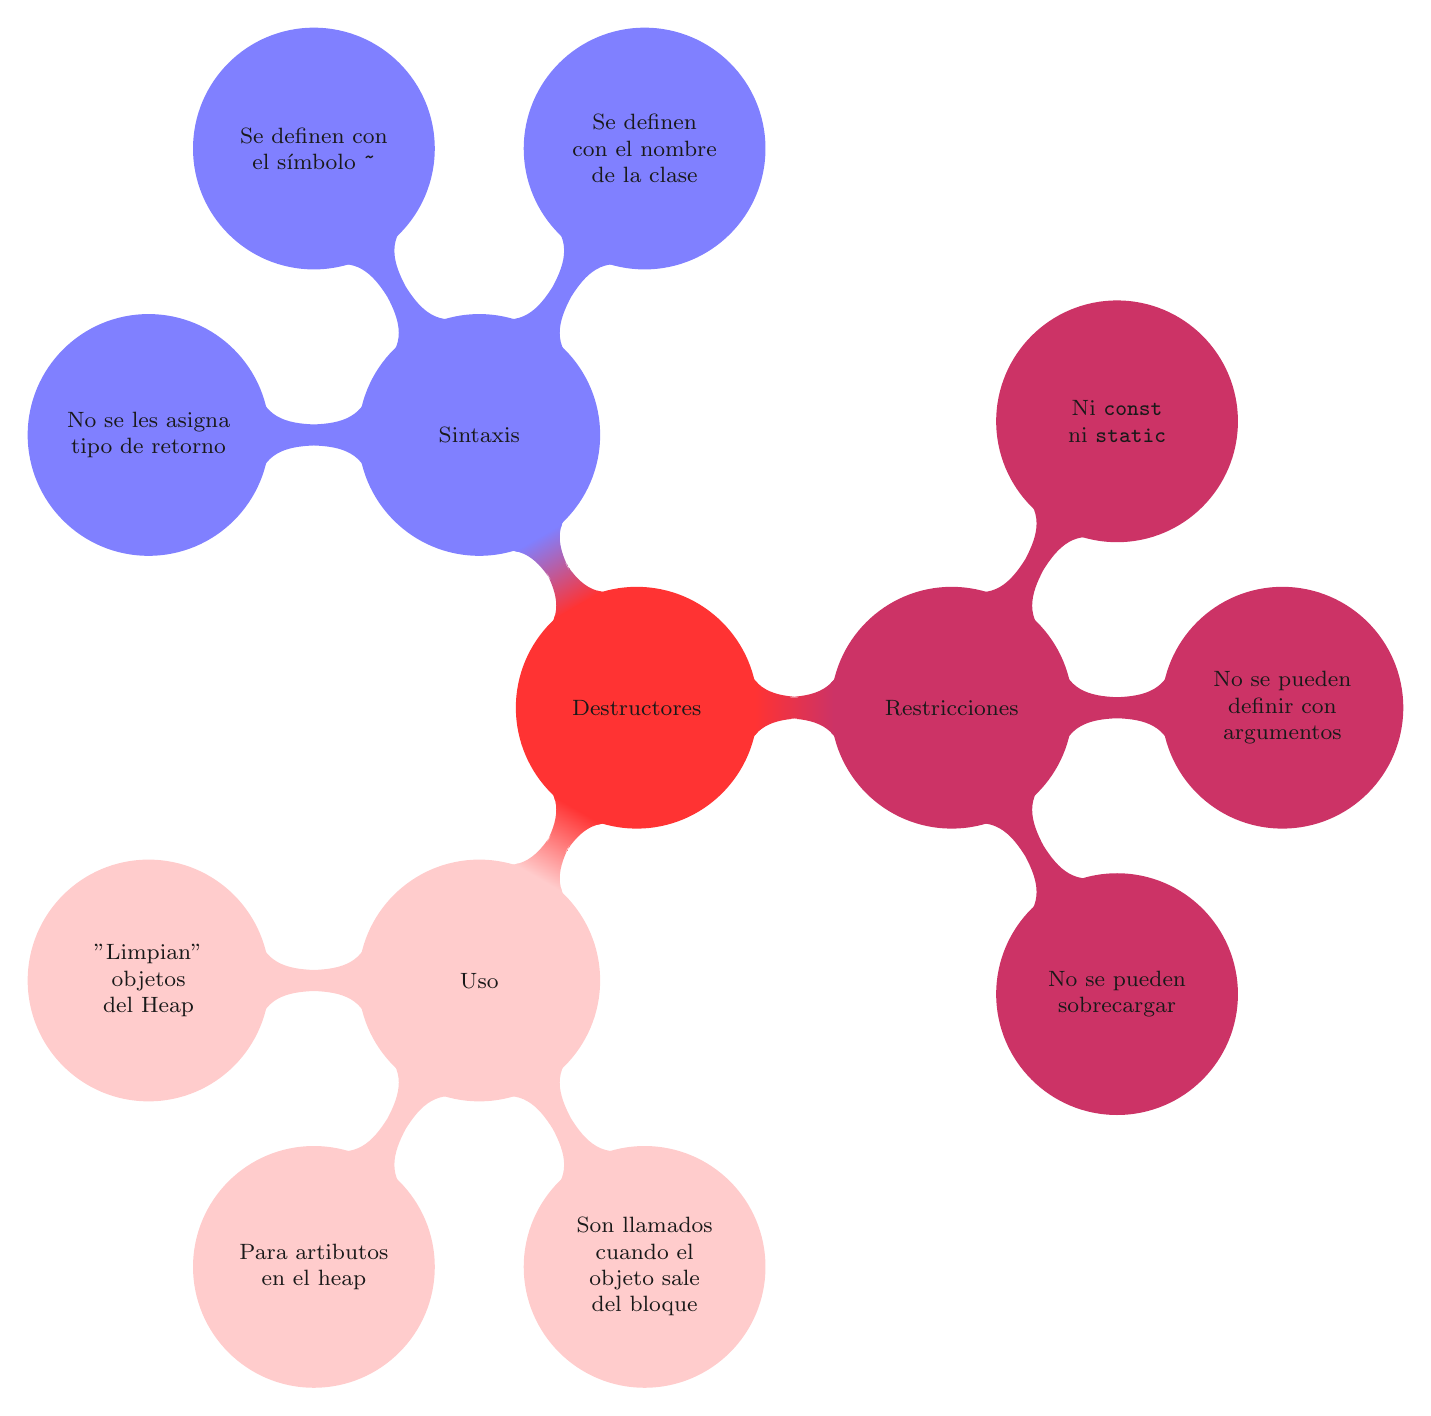
\begin{tikzpicture}[small mindmap, grow cyclic, every node/.style=concept, concept color=red!80, text=black!90, minimum size=3.0cm,
    level 1/.style={level distance=4.5cm,sibling angle=360/4},
    level 1/.style={level distance=4.0cm,sibling angle=360/3},
    level 2/.style={level distance=4.2cm,sibling angle=60},
    level 3/.style={level distance=3.5cm,sibling angle=60},
    ]
    \node{Destructores}
    child[concept color=pink!80] { node {Uso}
        child { node {"Limpian" objetos del Heap} }
        child { node {Para artibutos en el heap} }
        child { node {Son llamados cuando el objeto sale del bloque} }
    }
    child[concept color=purple!80] { node {Restricciones}
        child { node {No se pueden sobrecargar} }
        child { node {No se pueden definir con argumentos} }
        child { node {Ni \texttt{const} ni \texttt{static}} }
    }
    child[concept color=blue!50] { node {Sintaxis}
        child { node {Se definen con el nombre de la clase} }
        child { node {Se definen con el símbolo \texttt{\~} } }
        child { node {No se les asigna tipo de retorno} }
    }

    ;
\end{tikzpicture}
\end{center}
\end{document}
